% \vspace{20mm}
\newpage

\vspace*{\textheight}
\newpage

\noindent {\LARGE \textbf{Appendix}} \\

\section{Algorithm of \ourapproach}
\label{alg:codesim}

Algorithm~1 shows the pseudo-code of our prompting technique.

\begin{algorithm}[h]
\small
\caption{\tool}
\begin{algorithmic}[1]

\State $p \gets$ maximum number of planning steps
\State $d \gets$ maximum number of debugging steps \\
% \State $problem \gets$ problem to be solved\\

\For{$i \gets 1$ to $p$}
    \State \# Start of Planning Agent
    \State $plan \gets$ GeneratePlan($problem$)
    \State $feedback \gets$ ValidatePlan($problem$, $plan$)
    \If{$feedback$ is negative}
        \State $plan \gets$ RefinePlan($problem$, $plan$, $feedback$)
    \EndIf
    \State \# End of Planning Agent
    \\
    \State \# Start of Coding Agent
    \State $code \gets$ GenerateCode($problem$, $plan$) %\Comment{Coding Agent}
    
    \State $passed,\space log \gets$ test($code$, $sample\_io$) %Test code using sample IO\\
    \If{$passed$}
        \State Return $code$
    \Else
        % \State Pass $code$ to Debugging Agent
        \State \# Start of Debugging Agent
        \For{$j \gets 1$ to $d$}
            \State $code \gets$ DebugCode(\\
                \quad \quad \quad \quad \quad $problem$,\\
                \quad \quad \quad \quad \quad $plan$, \\
                \quad \quad \quad \quad \quad $code$, \\
                \quad \quad \quad \quad \quad $log$ \\
            \quad \quad \quad \quad) \\ %\Comment{Debugging Agent}
            \State $passed,\space log \gets$ test($code$, $sample\_io$)
            \If{$passed$}
                \State Return $code$
            \EndIf
        \EndFor
        \State \# End of Debugging Agent
    \EndIf
    \State \# End of Coding Agent
    \\
\EndFor
\State Return $code$
\end{algorithmic}
\end{algorithm}

\section{Exclusion of AgentCoder}
\label{app:elimination-of-agentcoder}
We have not included AgentCoder \cite{huang2023agentcoder} in our comparison due to reproducibility issues which undoubtedly plays a critical role in fair comparison as indicted in \citet{laskar-etal-2024-systematic}, as we were unable to replicate their results. In our attempts to reproduce their work on the HumanEval benchmark using ChatGPT, we achieved $56.7$\% accuracy after four iterations, consuming $11.9$ million tokens. When using GPT-4, we attained only $17.7$\% accuracy after two iterations, with $10.4$ million tokens consumed. The token consumption in both cases is significantly higher compared to MapCoder ($1.7$ million tokens with ChatGPT and $2.1$ million with GPT-4) and \toolnospace($0.89$ million tokens in ChatGPT and $0.85$ million in GPT-4). These two experiments resulted in a cost of approximately \$$500$ USD, but we were still unable to come close to AgentCoder's reported claims of $79.9$\% accuracy with ChatGPT and $96.3$\% with GPT-4.

Furthermore, we found unaddressed issues on their GitHub page (\href{https://github.com/huangd1999/AgentCoder/issues/8}{link}) related to reproducibility. Additionally, for the MBPP dataset, they used all test cases as public test cases (\href{https://github.com/huangd1999/AgentCoder/issues/3}{link}), which deviates from standard practices. As a result, we did not consider those results in our comparison either.

\section{Details Promptings of \tool}
\label{app:prompts}

The \emph{Planning Agent} interacts with the LLM three times to generate a plan. In the first API call, it instructs the LLM to comprehend the problem, generate an example problem, recommend a suitable algorithm, and finally produce the plan (Figure \ref{prompt:plan-generation}). In the second API call, the LLM is instructed to verify the plan through simulation (Figure \ref{prompt:plan-verification}). If the plan is satisfactory, it is returned by the agent. Otherwise, the LLM is called again to refine the plan based on the feedback from the simulation (Figure \ref{prompt:plan-refinement}).

The next step involves the \emph{Coding Agent}, which receives the plan from the \emph{Planning Agent} and uses the prompt outlined in Figure \ref{prompt:code-generation} to generate code.

If the code fails to pass the sample input/output, \tool activates its final agent, the \emph{Debugging Agent}, using the prompt shown in Figure \ref{prompt:debugging}.

These figures also include the rationale behind the inclusion of each sentence in the prompt.

\section{Example Problem}
We present a complete example of problem solving using \tool below:

% \onecolumn
% \newpage

\begin{figure*}[h]
    \centering
    \includegraphics[width=0.90\textwidth]{figures/steps/Plan-Generation.pdf}
    \caption{\emph{Planning Agent}: Prompt for Plan Generation. }
    \label{prompt:plan-generation}
\end{figure*} 

\begin{figure*}[h]
    \centering
    % \hspace*{-0.5cm}
    \includegraphics[width=0.90\textwidth]{figures/steps/Plan-Verification.pdf}
    \caption{\emph{Planning Agent}: Prompt for Plan Verification with the help of Simulation.}
    \label{prompt:plan-verification}
\end{figure*} 

\begin{figure*}[h]
    \centering% \hspace*{-0.5cm}
    \includegraphics[width=0.90\textwidth]{figures/steps/Plan-Refinement.pdf}
    \caption{\emph{Planning Agent}: Prompt for Plan Refinement.}
    \label{prompt:plan-refinement}
\end{figure*} 

\begin{figure*}[h]
    \centering% \hspace*{-0.5cm}
    \includegraphics[width=0.90\textwidth]{figures/steps/Code-Generation.pdf}
    \caption{\emph{Coding Agent}: Prompt for Code Generation.}
    \label{prompt:code-generation}
\end{figure*} 
\onecolumn

\begin{figure*}[h]
    \centering% \hspace*{-0.5cm}
    \includegraphics[width=0.90\textwidth]{figures/steps/Debugging.pdf}
    \caption{\emph{Debugging Agent}: Prompt for Debugging.}
    \label{prompt:debugging}    
\end{figure*}

% \onecolumn

\begin{tcolorbox}[breakable]
\label{app:example-problem}
    % !TEX root = main.tex

\begin{figure}[t]
\vspace{-1.5cm}
\begin{minipage}{0.34\textwidth}
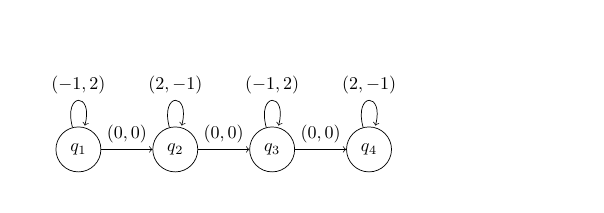
\begin{tikzpicture}[scale=0.25]
\usetikzlibrary{automata, positioning}
\scalebox{0.65}{
\node[state] (q1) {$q_1$};
\node[state, right=of q1] (q2) {$q_2$};
\node[state, right=of q2] (q3) {$q_3$};
\node[state, right=of q3] (q4) {$q_4$};

\path[->] (q1) edge [loop above] node[above] {$(-1,2)$} (q1) edge node[above] {$(0,0)$} (q2); 
\path[->] (q2) edge [loop above] node[above] {$(2,-1)$} (q2) edge node[above] {$(0,0)$} (q3);
\path[->] (q3) edge [loop above] node[above] {$(-1,2)$} (q3) edge node[above] {$(0,0)$} (q4);
\path[->] (q4) edge [loop above] node[above] {$(2,-1)$} (q4);
}
\end{tikzpicture}
\end{minipage}
\begin{minipage}{0.32\textwidth}
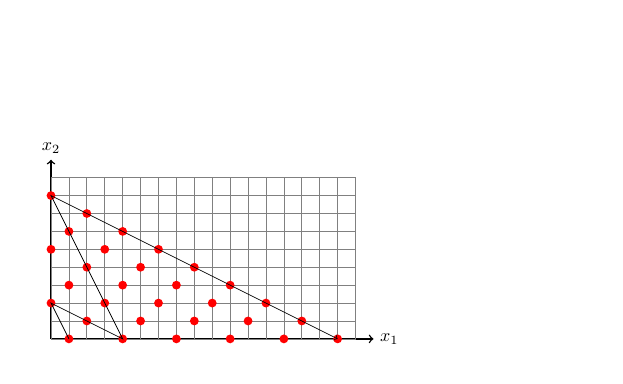
\begin{tikzpicture}[scale=0.35]
\scalebox{0.65}{
\draw[->, thick] (0, 0) -- (18, 0) node[right] {$x_1$};
\draw[->, thick] (0, 0) -- (0, 10) node[above] {$x_2$};

\draw[step=1, gray, thin] (0, 0) grid (17, 9);

\foreach \x in {1,4,7,10,13,16} \fill[red] (\x,0) circle (7pt);
\foreach \x in {2,5,8,11,14} \fill[red] (\x,1) circle (7pt);
\foreach \x in {0,3,6,9,12} \fill[red] (\x,2) circle (7pt);
\foreach \x in {1,4,7,10} \fill[red] (\x,3) circle (7pt);
\foreach \x in {2,5,8} \fill[red] (\x,4) circle (7pt);
\foreach \x in {0,3,6} \fill[red] (\x,5) circle (7pt);
\foreach \x in {1,4} \fill[red] (\x,6) circle (7pt);
\foreach \x in {2} \fill[red] (\x,7) circle (7pt);
\foreach \x in {0} \fill[red] (\x,8) circle (7pt);

\draw[->] (1,0) -- (0,2) -- (2,1) -- (4,0) -- (3,2) -- (2,4) -- (1,6) -- (0,8) -- (2,7) -- (4,6) -- (6,5) -- (8,4) -- (10,3) -- (12,2) -- (14,1) -- (16,0);
}
\end{tikzpicture}
\end{minipage}
\begin{minipage}{0.32\textwidth}
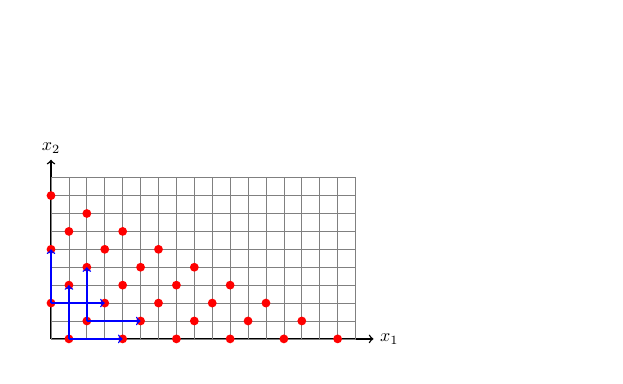
\begin{tikzpicture}[scale=0.35]
\scalebox{0.65}{
\draw[->, thick] (0, 0) -- (18, 0) node[right] {$x_1$};
\draw[->, thick] (0, 0) -- (0, 10) node[above] {$x_2$};

\draw[step=1, gray, thin] (0, 0) grid (17, 9);

\foreach \x in {1,4,7,10,13,16} \fill[red] (\x,0) circle (7pt);
\foreach \x in {2,5,8,11,14} \fill[red] (\x,1) circle (7pt);
\foreach \x in {0,3,6,9,12} \fill[red] (\x,2) circle (7pt);
\foreach \x in {1,4,7,10} \fill[red] (\x,3) circle (7pt);
\foreach \x in {2,5,8} \fill[red] (\x,4) circle (7pt);
\foreach \x in {0,3,6} \fill[red] (\x,5) circle (7pt);
\foreach \x in {1,4} \fill[red] (\x,6) circle (7pt);
\foreach \x in {2} \fill[red] (\x,7) circle (7pt);
\foreach \x in {0} \fill[red] (\x,8) circle (7pt);

\draw[->,blue,thick] (1,0) -- (4,0);
\draw[->,blue,thick] (1,0) -- (1,3);

\draw[->,blue,thick] (2,1) -- (5,1);
\draw[->,blue,thick] (2,1) -- (2,4);

\draw[->,blue,thick] (0,2) -- (3,2);
\draw[->,blue,thick] (0,2) -- (0,5);
}
\end{tikzpicture}
\end{minipage}
\caption{Left: 4-component \dvass $V_2$. 
Middle: the set $\reach_{q_4}(V_2, q_1(1,0))$ and a path $q_1(1,0) \tran q_4(16,0)$.
Right: bases 
%$A = \{(1,0),(2,1),(0,2)\}$ 
and periods 
%$P = \{(0,3),(3,0)\}$
 of an over-approximating semi-linear set $A+P^*$.}
\label{fig:zigzag}
\end{figure}

\begin{example}
For $k\geq 1$, let $V_k$ be a $(2k)$-component \dvass, where each component has just one state $q_i$
and one transition:
$(q_i, (-1,2), q_i)$ for odd $i$, and $(q_i, (2,-1), q_i)$ for even $i$.
Bridge transitions are $(q_i, (0,0), q_{i+1})$.
Figure~\ref{fig:zigzag} shows $V_2$ (left) and 
a path in $V_2$ from $s = q_1(1,0)$ to $t = q_4(16,0)$ together with 
the reachability set $\reach_{q_4}(V_2, s)$ (middle).
In general,
\begin{align} \label{eq:reachk}
X_k := \reach_{q_{2k}}(V_k, s) \ = \ \set{(x_1,x_2) \mid x_1+2x_2 \leq 4^k, \  x_1+2x_2 \equiv 1 \!\! \mod 3}.
\end{align}
Even if the size of the reachability set is 
exponential in $k$, for small $(x_1, x_2)$ it is periodic and the periods are small.
The set $X_k$ can be over-approximated by $A + P^*$ for $A = \set{(1,0),(2,1),(0,2)}$ and $P = \set{(0,3),(3,0)}$
(shown on the right of Figure~\ref{fig:zigzag}), namely for every $k\geq 1$ and $B\in\N$,
the set $X_k$ is \kanapka {$8$} {$B$}. 
For illustration, consider $Y := X_k \cap ((1,0) + P^*)$.
If $(1,0) + P^{\leq B} \subseteq X_k$ then $Y$ is a $B$-approximation
of $(1,0) + P^*$ with $\norm((1,0)), \norm(P) \leq 3 \leq 8$. 
Otherwise, there is some $(v_1, v_2) \in \big((1,0) + P^{\leq B}\big)\setminus X_k$, and
then $B$ is larger than $4^k$:
\[
%8B \geq 2(1 + 3B) \geq 2(v_1 + v_2) \geq v_1 + 2 v_2 > 
4^k < v_1 + 2 v_2 \leq 2(v_1 + v_2) \leq 2(1+3B) \leq 8B.
\]
Therefore by \eqref{eq:reachk}, each $(x_1,x_2) \in Y$ satisfies 
$\norm(x_1,x_2) = x_1 + x_2 \leq x_1 + 2x_2 \leq 4^k < 8B$, and thus
$Y$, seen as a union of singletons, is a union of 
linear sets with norm of base bounded by $8B$ and empty set of periods. 
In both cases, 
$Y$ is \kanapka {$8$} {$B$}. 
%The same intuition stays behind polynomial approximability of \dvass stated in Lemma~\ref{lem:2vass-sandwich}.
\end{example}
\end{tcolorbox}
\twocolumn  % Switch back to two-column mode